%!TEX ROOT = thesis.tex
\chapter{Framework Overview}

\section{Introduction}
In order to tackle the issues discussed in the earlier through the literature review as well as the various motivations, the theoretical framework is laid as to provide a conceptual schema on how to break the rather huge and intricate challenge into multiple bite sized puzzles. This chapter is organized as such, first, the overview of the framework used in this work is described in Section \ref{section:framework}, followed by some reoccurring key concepts throughout this work in Section \ref{section:keyconcepts}. Next, the description of the dataset used is described in Section \ref{section:dataset_used} and finally, this chapter concludes with the experimental methodology applied in this work (see Section \ref{sec:expmethodology}). 


\section{Framework Overview}
\label{section:framework}
In this section, a high level overview of the fundamental processing step along with two suggested core components for vehicle semantic extraction and retrieval is provided. The groundwork described in this work abides to the typical top-down approach used in Intelligent Transportation System (ITS) where the video data is subjected to background subtraction, followed by blob filtering, vehicle detection as well as vehicle tracking is as described in \cite{lim2017}. 

The semantic information from the vehicle blobs are then extracted and stored in the database. With the vehicle specific semantics stored in the database, retrieval engines were designed to enabled users to easily retrieve the stored information. Both retrieval engines features a graphical user interface which allowed users to enter the queries by drawing the desired trajectory as well as entering other crucial information which would assist in identifying the targeted video shot.


\begin{figure}[hbt!]\centering
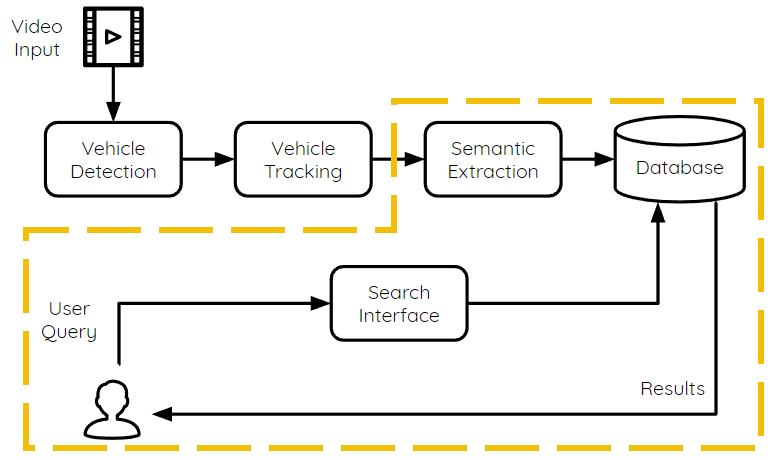
\includegraphics[width=.9\textwidth]{image/framework_new.PNG}
\caption{Framework Diagram, Contribution in Highlighted Border}
\label{fig:framework}
\end{figure}


In this work, two frameworks were suggested and used for the vehicle semantic extraction and retrieval process. Both of which utilizes an underlying distinctive approach, with the same end goal in mind, which is the retrieval of desired video snippets which closely resembles a user described query. For each of these frameworks, the formulation of idea, steps and process involved are described in this chapter. As there are various solutions proposed in this work, solutions which are common to both core frameworks is also provided. As a whole, the end-to-end framework can be visualized using Figure \ref{fig:framework} where the main contribution of this work is highlighted in yellow border. 

\subsection{LSH-Inspired Retrieval Framework}
The first of the two frameworks suggested in this work is the \textit{LSH-Inspired Retrieval Framework}. Locality-Sensitve Hashing (LSH) refers to a technique used for dimensionality reduction, typically to perform hashing on a set of documents so that documents with similar properties are mapped and clustered to similar locality or neighbourhood. This technique excels especially when working with high dimensional data such as video data in this work.

By building on top of the fundamental processing step, the semantics from each vehicle blobs are extracted

\subsection{Chamfer Distance based Framework}




\section{Key Concepts}
\label{section:keyconcepts}
In this section, a reoccurring key concept used in the proposed method is discussed as to provide a high level understanding. 

\cc{try to expound more on this part}


\subsection{Quantization}

The use of quantization in the mathematical and digital signal processing field is no longer a new concept. However, digital signal processors are limited by natural boundaries such as hardware limitations, and are only able to compute and perform arithmetic operations within a limited range \cite{spors_2018}. The use of quantization refers to the process of mapping and projecting a set of large values which are often continuous or analog in nature into a set of discrete and finite values. 

\begin{figure}[hbt!]\centering
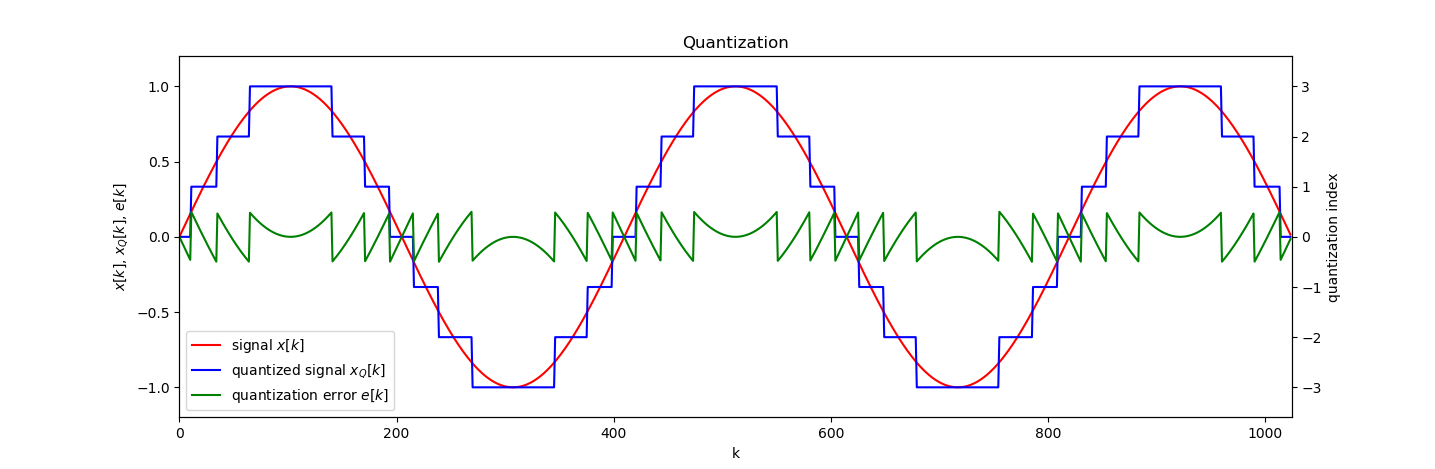
\includegraphics[width=\textwidth]{image/general/quantization.png}
\caption{Quantization}
\end{figure}


The use of quantization enables reduction in memory usage (compression) as well as to reduce computational cost which leads to faster processing speed. However, since quantization is a many-to-few mapping operation, hence, the operation is considered irreversible without prior knowledge of the loss. Nevertheless, the output discrete signal can closely resemble the input continuous signal depending on the number of quantization index used.   

In the proposed method, the quantization technique was extended further into a three dimensional space where the 3D space is quantized into a set of discrete and finite values to ease the calculation and manipulation of data in the both the video data as well as the color space. 

\begin{equation}\centering
\label{eq:quantization}
x_Q[k] = g( \mspace{3mu}\lfloor \mspace{3mu}f(x[k]) \mspace{3mu}\rfloor\mspace{3mu})
\end{equation} 

\vspace{-3em}


\begin{equation}\centering
\label{eq:quantizationerror}
e[k] = x_Q[k] - x[k]
\end{equation}


In order to expound on the quantization process, a mathematical model of this process can be formulated as such. Consider a continuous signal $x[k]$ whose quantized signal, $x_Q[k]$, is desired. The functions $f (\mspace{3mu} \cdot  \mspace{3mu})$ \& $g (\mspace{3mu} \cdot  \mspace{3mu})$ can be thought of as a real-value mapping function while the $\lfloor \mspace{3mu} \cdot  \mspace{3mu} \rfloor$ represents a rounding function. As previously mention, this process is considered irreversible with prior knowledge of the loss, in this case, the quantization error, $e[k]$, can be computed using the Equation \ref{eq:quantizationerror}. 

\subsection{Distance Measure}
\label{section:distancemeasures}

The use of distance metrics is another reoccurring key concept in the proposed method. While distance measure is commonly used in computer science as well as the mathematics field, there are numerous metrics suggested by different authors which are applicable and useful in different scenarios.   

In the proposed method, the use of distance metrics allows the author to measure the performance of the proposed algorithms. A simple example of how distance metrics is applied in the proposed method can be illustrated using Figure \ref{fig:distanceMeasure} where the distance between two lines signifies the dissimilarity between them. 



\begin{figure}[hbt!]\centering
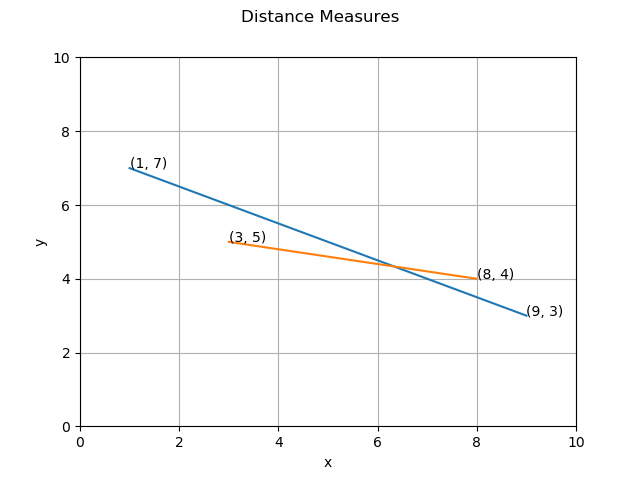
\includegraphics[width=.7\textwidth]{image/general/distance.png}
\caption{Example of Distance Measure}
\label{fig:distanceMeasure}
\end{figure}

As different distance measure metrics are favourable in different scenarios, a good distance measure when used in a carpark scene is essential when comparing a significantly extensive set of vehicle trajectories during the retrieval process.   

Again, this concept was further extended into a multi-dimensional space such as the colors space, where the similarity between two or more colors was measured using different distance metrics to evaluate the performance of each metric. 



\subsection{Color Model}

While humans' visible spectrum $(400nm - 700nm)$ can be represented using the respective wavelengths,  in order to describe these values in a 

\cc{to fill up... talk about color space and why}
%http://markkness.net/colorpy/ColorPy.html

\begin{figure}[hbt!]\centering
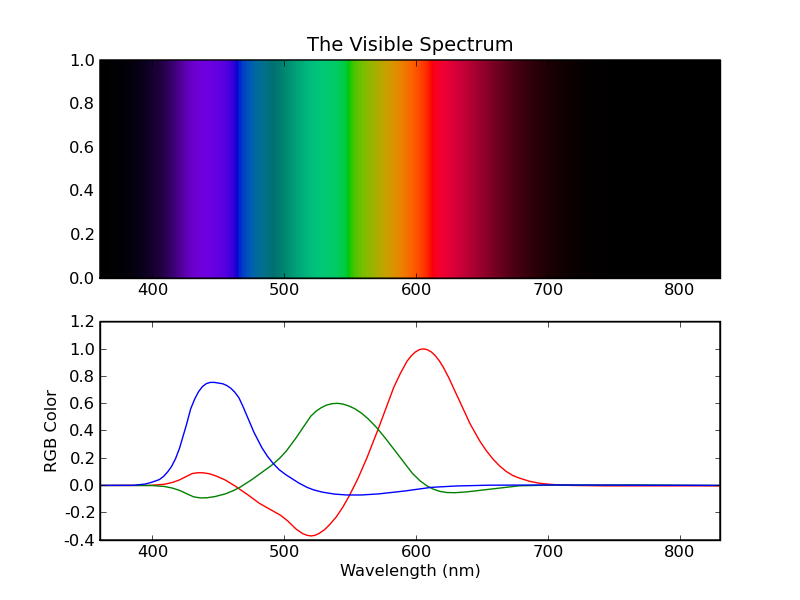
\includegraphics[width=.7\textwidth]{image/general/VisibleSpectrum.png}
\caption{RGB Values and their corresponding spectrum}
\label{fig:visibleSpectrum}
\end{figure}





\section{Dataset}
\label{section:dataset_used}

In view of testing the proposed framework for large-scale extraction and retrieval of video semantics, a new collection of video dataset was gathered. A stationary cloud-enabled web camera was set up on the fourth floor of a building with a window facing a piece of private carpark area. Figure \ref{fig:camerasetup} depicts the camera setup overcasting the carpark area. 

The aforementioned setup was done to mimic a typical camera setup which tower over a piece of outdoor carpark lot that are found in the wild. 


\begin{figure}[hbt!]\centering
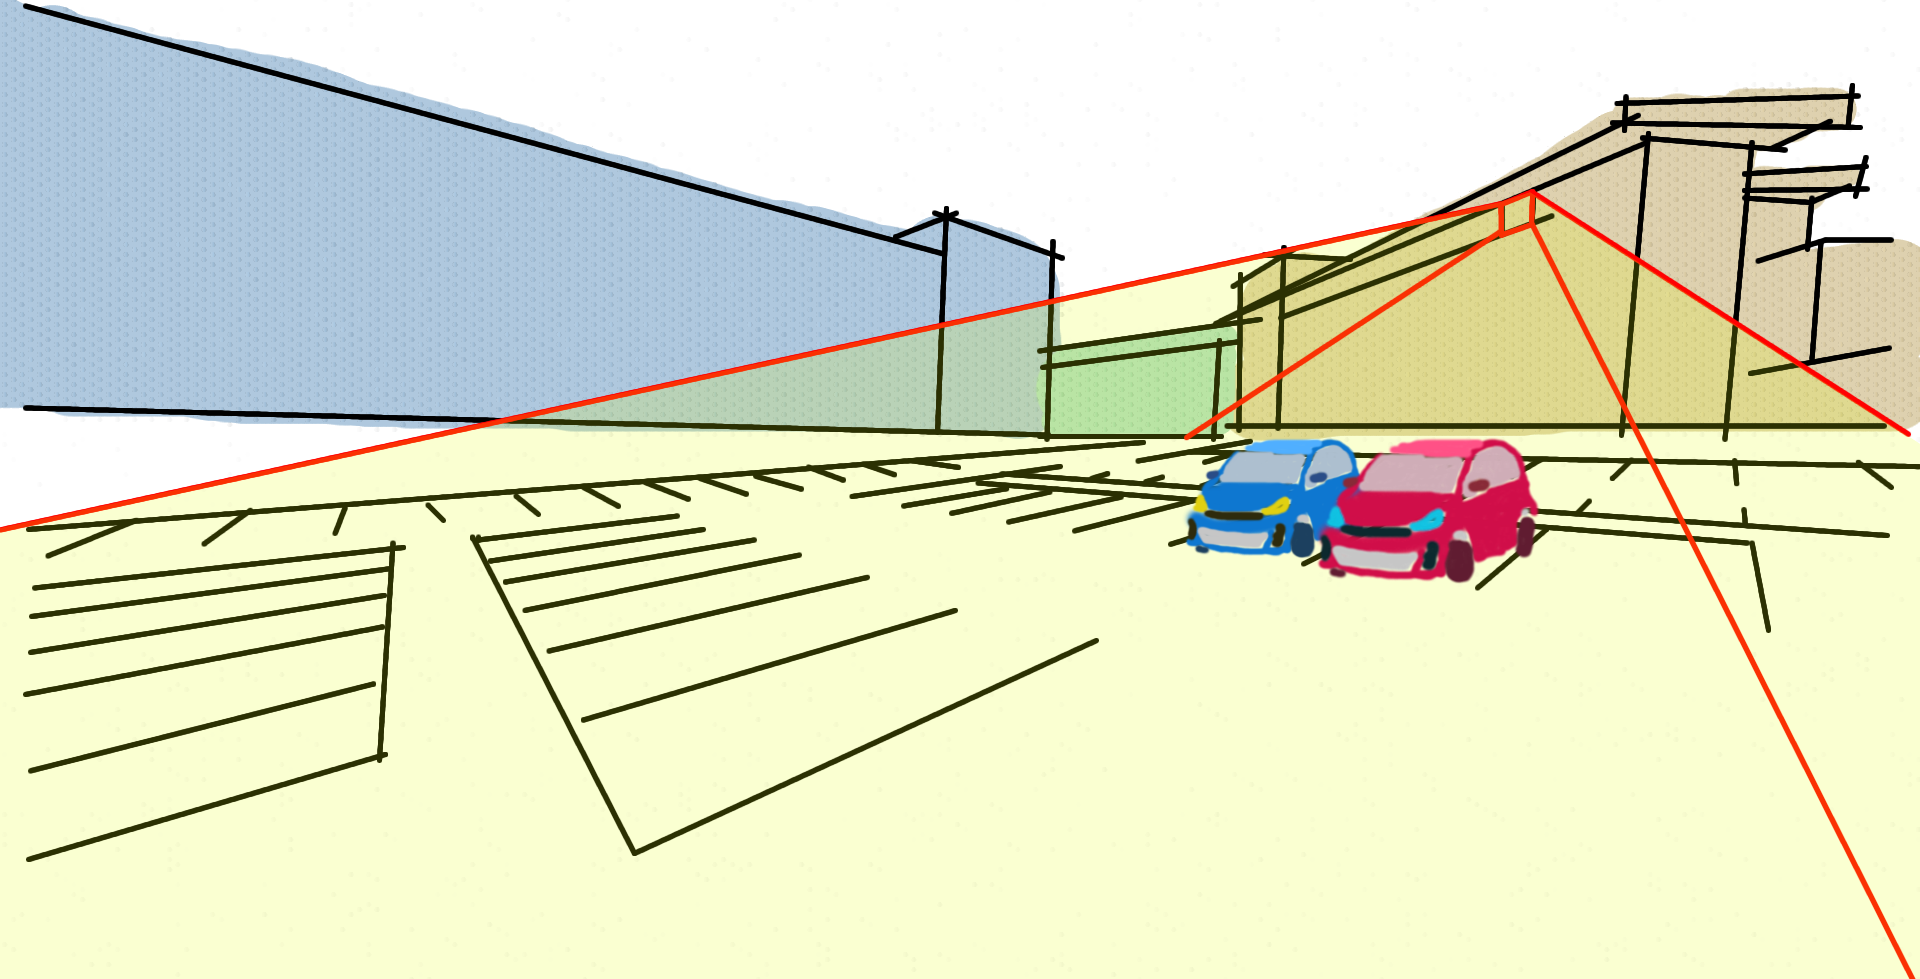
\includegraphics[width=.8\textwidth]{image/fcicarpark2.png}
\caption{Camera setup to capture the carpark from the fourth floor}
\label{fig:camerasetup}
\end{figure}


\begin{figure}[!hbt]\centering
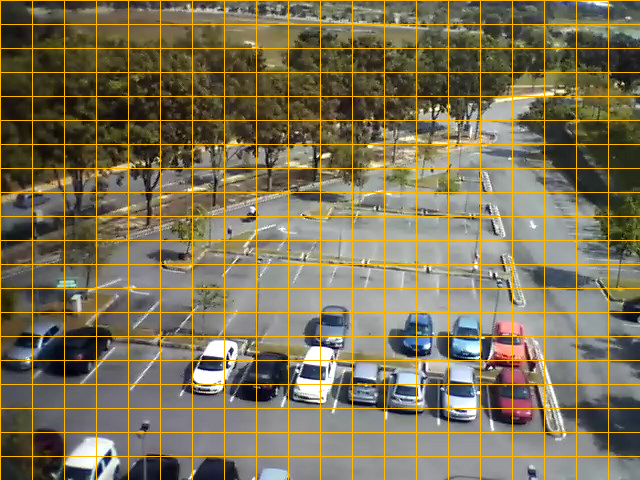
\includegraphics[width=.7\textwidth]{image/general/grids.png}
\caption{View from camera setup; 20$\times$20 Grids}
\label{fig:viewfromcamera}
\end{figure}


Through the camera's web interface, this device was set to record on weekdays from Monday through Friday, starting from 08:30 in the morning up until 18:30 in the evening, with a total of 10 hours was recorded each day. Among the important settings, each recorded video clip was set to have a maximum length of 6 minutes, and hence, 10 video clips every hour, and a total of 100 at the end of each day. The recorded video clips were saved into the external microSD memory card. At the end of each day, the data was then copied over to a server via a script. However, due to glitches that occurred during the recording process, some of the video clips were cut off abruptly. Hence, some of the days do not contain the full 10 hours video clips. 

\begin{table}[]\centering
\begin{tabular}{ll}
Camera Model: & Dlink DSC-942L        \\
Resolution:   & 640$\times$480 pixels \\
Frame rate:   & 10 $fps$             \\
Format:       & H.264 / MPEG-4 AVC    \\
Naming Convention: & $CCYYMMDD\_HHMMSS.mp4$
\end{tabular}
\vspace{1em}
\caption{Camera details}
\end{table}

\begin{figure}[htb!]
  \centering

\begin{tabular}{cc}
 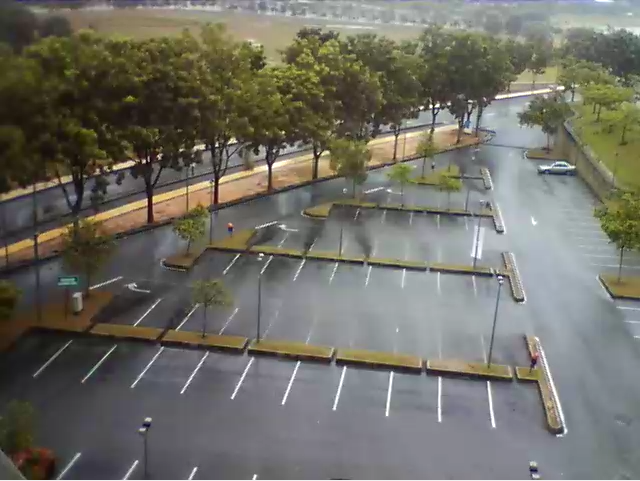
\includegraphics[width=0.4\linewidth]{image/general/rain.PNG} &  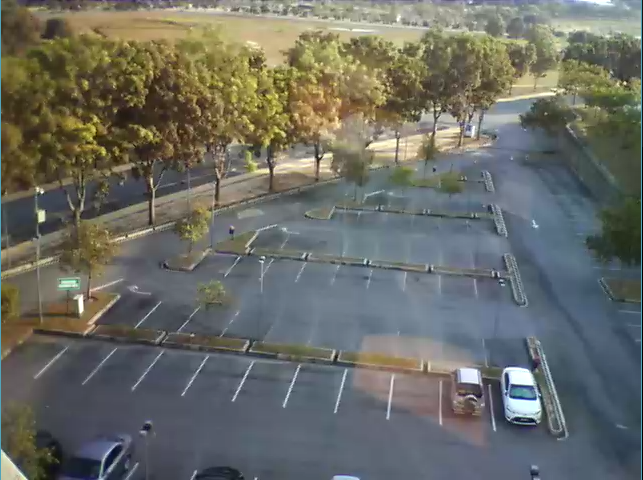
\includegraphics[width=0.4\linewidth]{image/general/reflection.PNG}\\ 
\begin{tabular}{c}(a) Rainy day with \\ reflective surface\end{tabular} & \begin{tabular}{c}(b) Reflection on the \\carpark from the window\end{tabular} \\
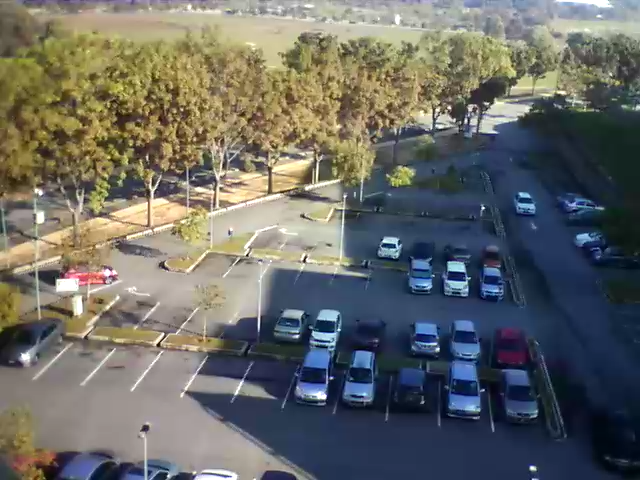
\includegraphics[width=0.4\linewidth]{image/general/shadow.png} &  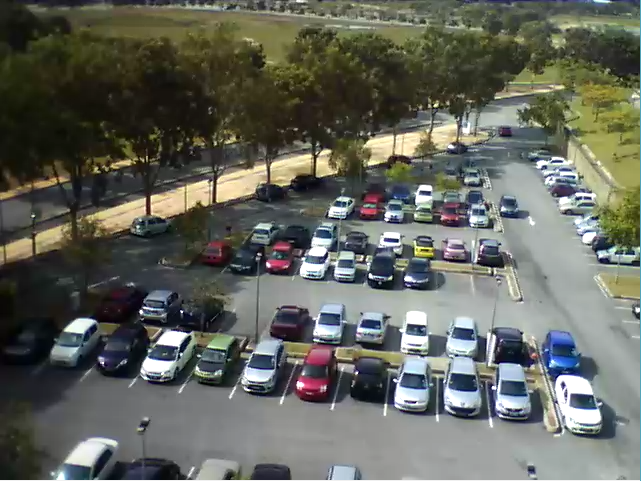
\includegraphics[width=0.4\linewidth]{image/general/shadow2.png}\\
\begin{tabular}{c}(c) Severe shadow over \\ the car park (08:48AM)\end{tabular} & \begin{tabular}{c}(d)  Severe shadow over \\ the car park (04:06PM)\end{tabular}
\end{tabular}


\caption{Noisy data within the collected dataset} \label{fig:weather}
\end{figure}


This setup was left to record data over the course of several months with various weather conditions, lighting conditions as well as a diverse set of carpark scenes which includes peak hours with plenty of vehicles along with the off-days. In addition to that, this setup covers a total of over 45 parking lots which excludes parking lots which are too small or occluded to be considered. Figure \ref{fig:weather} exhibits the various weather condition and noise which were recorded sporadically throughout the dataset.





\section{Experimental Methodology}
\label{sec:expmethodology}

In the subsequent chapters, the detailed descriptions of the proposed vehicle semantic extraction algorithm as well as the retrieval engine modules will be provided. In this section, the methodology and the experimental setup is briefly discussed to provide a overview on how the experiments will be performed in this work.

As the performance of the proposed method is essential towards end users, each of the proposed algorithm in the framework is evaluated with the help of volunteers. Even though the fundamental framework was adopted from \cite{lim2017} without changes on the underlying algorithm, errors which were propagated from the Vehicle Detection and Vehicle Tracking modules were not overlooked nor discarded during the evaluation of the subsequent modules in the pipeline. This was done intentionally to provide an end-to-end assessment of the framework. 

The proposed methods were implemented and evaluated on an Intel i7 machine with 16GB RAM, GeForce GTX 1060 GPU. As the main focal point in this proposed method revolves around the semantic extraction of vehicle color along with the vehicle trajectory, each of these component in the pipeline were assessed and evaluated individually in order to obtain and understand the performance, effectiveness as well as the weakness of the proposed methods. This, in turn, provides a deeper understanding and opportunities for improvements as well as future works. 

While the collected dataset comprised of several months of data, only two days of data were manually fully annotated by several annotators and cross-checked to arrive at a consensus. These manually annotated dataset included the total number of vehicles with their corresponding color categories, along with that, the total number of vehicles performing $TQ1$ \& $TQ2$ (see Figure \ref{fig:versionOneInterface}) which were used the evaluation of \versionOne was recorded. 

However, as with any large scale retrieval engine, for all intents and purposes, it is not feasible to annotate a huge amount of ground truth manually as it is a labour intensive, mundane and time consuming process. Hence in \versionTwo, one month of data was processed and evaluated without the manual annotations of all the events. Instead, the best practice used in evaluating a large scale retrieval engine was used to document the evaluation process. To do that, the relevance of each results was evaluated by the volunteers who described the test queries. 

